\documentclass{article}

% Use neurips_2024 style (download separately if needed)
% For now, use a clean article format
\usepackage[utf8]{inputenc}
\usepackage[T1]{fontenc}
\usepackage{hyperref}
\usepackage{url}
\usepackage{booktabs}
\usepackage{amsfonts}
\usepackage{amsmath}
\usepackage{amssymb}
\usepackage{nicefrac}
% \usepackage{microtype}  % Disabled due to font expansion issues
\usepackage{graphicx}
\usepackage{xcolor}
% Algorithm packages - use algorithmicx if available, else skip
% \usepackage{algorithm}
% \usepackage{algorithmic}
\usepackage{subcaption}

% Page setup
\usepackage[margin=1in]{geometry}

% Custom commands
\newcommand{\fu}{\mathbf{f}_u}
\newcommand{\W}{\mathbf{W}}
\newcommand{\x}{\mathbf{x}}
\newcommand{\proj}{\text{proj}}
\newcommand{\R}{\mathbb{R}}

\title{Targeted Direction Unlearning: \\
Surgical Fact Removal via Interpretable Projections}

\author{
  Anonymous Authors
}

\date{}

\begin{document}

\maketitle

\begin{abstract}
We introduce \textbf{Targeted Direction Unlearning (TDU)}, a novel method for removing specific factual knowledge from large language models. 
Unlike gradient-based unlearning methods that require iterative optimization, TDU discovers the \emph{direction} in activation space that encodes a target fact, then surgically removes it via rank-one projection. 
Our key insight is that factual knowledge is encoded as approximately linear directions in MLP output spaces, and projecting out these directions effectively ``forgets'' the fact while preserving unrelated knowledge.

We evaluate TDU on the CounterFact benchmark across GPT-2, Pythia-410M, and Pythia-1B models. 
Our experiments show that: (1) facts are consistently encoded in early-middle layers (layers 1-4), (2) TDU achieves competitive efficacy with state-of-the-art methods while being 10x faster, and (3) the discovered directions are interpretable---directions for related facts show high cosine similarity.
TDU provides a practical and interpretable approach to targeted knowledge removal, with implications for privacy compliance, factual updates, and model safety.
\end{abstract}

%% ============================================
%% INTRODUCTION
%% ============================================
\section{Introduction}
\label{sec:introduction}

Large language models (LLMs) have demonstrated remarkable capabilities across a wide range of tasks, from question answering and code generation to complex reasoning. However, these models inevitably encode factual knowledge that may become outdated, contain sensitive personal information, or pose safety risks. The ability to selectively remove or modify specific knowledge from a trained model---without expensive retraining from scratch---has thus emerged as a critical capability for responsible deployment of LLMs.

The need for targeted knowledge removal arises from multiple practical concerns. Privacy regulations such as GDPR establish a ``right to be forgotten,'' requiring systems to delete personal information upon request. Models may memorize copyrighted content, confidential data, or information that enables harmful applications. Furthermore, the factual knowledge encoded during training inevitably becomes stale: world leaders change, scientific understanding evolves, and corporate affiliations shift. In all these cases, practitioners require methods to surgically excise specific facts while preserving the model's broader capabilities.

Existing approaches to knowledge editing and unlearning fall broadly into two categories. The first class of methods employs gradient-based fine-tuning, using carefully constructed loss functions to ``unlearn'' targeted information. While conceptually straightforward, these approaches suffer from several limitations: they require multiple optimization steps, risk catastrophic forgetting of unrelated knowledge, and provide little insight into how or where the target knowledge was stored. The optimization process treats the model as a black box, offering no guarantees about the completeness of removal or interpretability of the intervention.

The second category comprises weight-editing methods such as ROME and MEMIT, which directly modify model parameters to insert, update, or remove factual associations. These methods identify specific layers where factual recall occurs and compute rank-one updates to the MLP weights. While more efficient than gradient-based approaches, they remain focused on editing the \emph{output} of factual queries rather than understanding the underlying \emph{representation} of facts within the model. The interventions are derived from input-output relationships and do not directly engage with the geometric structure of the model's internal representations.

A significant gap thus exists in the current landscape: we lack methods that are simultaneously \emph{interpretable}, \emph{surgical}, and \emph{efficient}. An ideal unlearning method would identify precisely where and how a fact is encoded, remove it through a minimal and understandable intervention, and do so without iterative optimization or risk of collateral damage. Such a method would not only serve practical needs but also advance our scientific understanding of how LLMs represent knowledge.

In this work, we introduce \textbf{Targeted Direction Unlearning (TDU)}, a novel approach that addresses these desiderata. TDU is grounded in the linear representation hypothesis---the empirical observation that many concepts and features are encoded as directions in a model's activation space. We hypothesize that specific factual associations similarly correspond to identifiable directions, and that projecting out these directions can selectively remove the associated knowledge.

Our method proceeds in two stages. First, we \emph{discover} the direction in activation space that encodes a target fact. We achieve this by constructing contrastive prompts that isolate the factual association of interest and analyzing the resulting activation patterns. This yields an interpretable geometric object---a direction vector---that we can inspect, visualize, and validate. Second, we \emph{remove} the fact by applying a rank-one projection that orthogonalizes the relevant activation subspace with respect to the discovered direction. This intervention is surgical: it modifies the model's computations only along the specific direction associated with the target fact.

TDU offers several advantages over existing approaches:

\begin{itemize}
    \item \textbf{Interpretability:} The discovered direction provides direct insight into how the model encodes the target fact. We can examine which tokens activate this direction, how it evolves across layers, and whether it generalizes across paraphrased queries.
    
    \item \textbf{Surgical precision:} The rank-one projection is a minimal intervention that affects only the subspace encoding the target fact. Unlike gradient-based methods, there is no optimization that might inadvertently modify unrelated knowledge.
    
    \item \textbf{Efficiency:} TDU requires only forward passes to discover the direction and a single weight modification to implement the projection. No iterative optimization is needed, making the method substantially faster than fine-tuning approaches.
    
    \item \textbf{Verifiability:} Because the intervention is geometrically interpretable, we can verify its effects through activation analysis. We can confirm that the target direction has been nullified while other directions remain intact.
\end{itemize}

We evaluate TDU on standard knowledge unlearning benchmarks, measuring both the efficacy of fact removal and the preservation of unrelated capabilities. Our experiments demonstrate that TDU achieves competitive unlearning performance while providing unprecedented interpretability into the removal process. We further analyze the discovered directions, revealing insights into how factual knowledge is organized within LLM representations.

The remainder of this paper is organized as follows. Section~\ref{sec:related_work} surveys related work on knowledge editing, unlearning, and representation analysis in LLMs. Section~\ref{sec:method} presents the TDU method in detail, including our direction discovery procedure and projection-based removal mechanism. Section~\ref{sec:experiments} describes our experimental setup and presents results on unlearning benchmarks. Section~\ref{sec:analysis} provides interpretability analyses of the discovered directions. Finally, Section~\ref{sec:conclusion} discusses limitations and directions for future work.


%% ============================================
%% RELATED WORK
%% ============================================
\section{Related Work}
\section{Related Work}
\label{sec:related_work}

Our work draws on four main research areas: knowledge editing, machine unlearning, mechanistic interpretability, and sparse feature discovery. We position TDU at the intersection of these fields, leveraging interpretability insights to achieve efficient, targeted unlearning.

\subsection{Knowledge Editing in LLMs}

Knowledge editing methods aim to modify specific facts stored in language models without full retraining. \citet{meng2022locating} introduced ROME (Rank-One Model Editing), which uses causal tracing to identify that factual associations are primarily stored in middle-layer MLP modules. ROME then performs a rank-one update to the MLP weights to overwrite targeted facts. \citet{meng2023massediting} extended this to MEMIT (Mass-Editing Memory in Transformers), enabling simultaneous editing of thousands of facts by distributing updates across multiple layers.

While these methods achieve precise factual modifications, they have notable limitations. First, they require identifying the exact layer(s) where a fact is stored, which can vary across facts and models. Second, the weight modifications are not inherently interpretable---it is difficult to verify what other behaviors may be affected. Third, these methods are designed for editing rather than removal; adapting them to unlearning requires careful consideration of what the ``new'' fact should be. Our approach sidesteps these issues by operating in activation space rather than weight space, providing both interpretability and flexibility.

\subsection{Machine Unlearning}

Machine unlearning seeks to remove the influence of specific training data from a model \citep{bourtoule2021machine, cao2015towards}. For LLMs, common approaches include gradient ascent on the forget set \citep{jang2023knowledge, yao2024large}, which maximizes loss on targeted examples to ``unlearn'' them. Other methods employ fine-tuning on retain sets \citep{maini2024tofu}, knowledge distillation from a model without the target data \citep{chundawat2023can}, or preference optimization to steer away from undesired outputs \citep{zhang2024negative}.

These approaches face a fundamental tension: aggressive unlearning damages general model capabilities, while conservative unlearning leaves residual knowledge. Gradient-based methods are particularly prone to catastrophic forgetting on retain sets \citep{shi2024muse}. Moreover, most unlearning methods require multiple training epochs, making them computationally expensive. TDU addresses these challenges through targeted intervention on specific directions, enabling surgical removal with minimal collateral damage and no gradient-based optimization at inference time.

\subsection{Mechanistic Interpretability}

Mechanistic interpretability aims to reverse-engineer neural network computations into human-understandable components \citep{olah2020zoom, elhage2021mathematical}. Key techniques include activation patching \citep{vig2020investigating, meng2022locating}, which isolates the causal effect of specific activations by transplanting them between forward passes, and causal tracing \citep{pearl2009causality, meng2022locating}, which tracks how information flows through the network.

A central finding is the linear representation hypothesis: neural networks often encode high-level concepts as directions in activation space \citep{mikolov2013linguistic, park2023linear, nanda2023emergent}. This has been demonstrated for diverse concepts including sentiment \citep{tigges2023linear}, truthfulness \citep{marks2023geometry, li2024inference}, and factual associations \citep{hernandez2024linearity, geva2023dissecting}. Our method directly leverages this insight---if facts are encoded as directions, we can identify and suppress these directions to achieve unlearning. TDU's $\mathbf{f}_u$ vectors can be viewed as learned ``fact directions'' optimized specifically for removal.

\subsection{Sparse Autoencoders and Feature Discovery}

Sparse autoencoders (SAEs) have emerged as a powerful tool for discovering interpretable features in neural network activations \citep{cunningham2023sparse, bricken2023monosemanticity}. SAEs learn overcomplete dictionaries where each dictionary element ideally corresponds to an interpretable concept, with activations decomposed as sparse combinations of these features. This approach has revealed interpretable features for diverse concepts ranging from syntax to world knowledge \citep{templeton2024scaling, gao2024scaling}.

Our unlearning directions $\mathbf{f}_u$ share conceptual similarities with SAE features: both are directions in activation space that capture specific semantic content. However, while SAE features emerge from unsupervised reconstruction objectives, our directions are optimized explicitly for targeted fact removal. This task-specific optimization allows $\mathbf{f}_u$ to capture precisely the components relevant for unlearning, potentially spanning multiple SAE features or capturing aspects that SAEs miss. Furthermore, our directions require no auxiliary decoder network and can be applied efficiently at inference time through simple projection operations.


%% ============================================
%% METHOD
%% ============================================
\section{Method: Targeted Direction Unlearning}
\label{sec:method}

We present \emph{Targeted Direction Unlearning} (TDU), a method for selectively removing factual knowledge from large language models through learned directional interventions. Our approach is grounded in the linear representation hypothesis~\citep{park2023linear,nanda2023emergent}, which posits that concepts are encoded as directions in neural network activation spaces. We exploit this structure to identify and ablate the specific directions responsible for encoding targeted facts.

\subsection{Problem Formulation}
\label{sec:problem}

Consider a pretrained language model $\mathcal{M}$ with parameters $\bm{\theta}$ consisting of $L$ transformer layers. Let $\mathcal{D}_{\text{forget}} = \{(x_i, y_i)\}_{i=1}^{N_f}$ denote the \emph{forget set}---a collection of prompt-completion pairs representing factual knowledge to be removed. Similarly, let $\mathcal{D}_{\text{retain}} = \{(x_j, y_j)\}_{j=1}^{N_r}$ denote the \emph{retain set}, representing knowledge and capabilities that must be preserved.

The objective of targeted unlearning is to produce modified parameters $\bm{\theta}'$ such that:
\begin{enumerate}
    \item \textbf{Forgetting:} The model can no longer generate or assign high probability to targets in $\mathcal{D}_{\text{forget}}$.
    \item \textbf{Retention:} Model behavior on $\mathcal{D}_{\text{retain}}$ (and general capabilities) remains unchanged.
\end{enumerate}

We focus on factual associations of the form $(s, r, o)$ representing subject-relation-object triples (e.g., ``The Eiffel Tower is located in Paris''). Following prior work on knowledge localization~\citep{meng2022locating,geva2023dissecting}, we hypothesize that such facts are primarily encoded in the MLP sublayers of transformer blocks, where the output activations contain linearly separable directions corresponding to specific factual content.

\subsection{Directional Intervention Framework}
\label{sec:direction}

The core insight of TDU is that removing a fact corresponds to ablating a specific direction in the MLP output space. For each layer $\ell \in \{1, \ldots, L\}$, let $\mathbf{h}^{(\ell)} \in \mathbb{R}^d$ denote the MLP output activation at a given token position, where $d$ is the model's hidden dimension.

We seek to learn a unit vector $\mathbf{f}_u^{(\ell)} \in \mathbb{R}^d$ (with $\|\mathbf{f}_u^{(\ell)}\|_2 = 1$) that captures the direction encoding the targeted fact at layer $\ell$. The intervention operation projects out this direction from the MLP output:
\begin{equation}
    \tilde{\mathbf{h}}^{(\ell)} = \mathbf{h}^{(\ell)} - \left(\mathbf{f}_u^{(\ell)\top} \mathbf{h}^{(\ell)}\right) \mathbf{f}_u^{(\ell)} = \left(\mathbf{I} - \mathbf{f}_u^{(\ell)} \mathbf{f}_u^{(\ell)\top}\right) \mathbf{h}^{(\ell)}
    \label{eq:projection}
\end{equation}
where $\mathbf{I} \in \mathbb{R}^{d \times d}$ is the identity matrix. This orthogonal projection removes the component of $\mathbf{h}^{(\ell)}$ lying along $\mathbf{f}_u^{(\ell)}$ while preserving all orthogonal components.

\paragraph{Learning the Direction.}
We parameterize $\mathbf{f}_u^{(\ell)}$ as a learnable vector and optimize it to maximize the forgetting effect while minimizing collateral damage. Let $\mathcal{L}(x, y; \bm{\theta})$ denote the cross-entropy loss of the model on input-target pair $(x, y)$. We define two loss terms:

\textbf{Intervened loss} $\mathcal{L}_{\text{int}}$: The loss computed with directional interventions applied:
\begin{equation}
    \mathcal{L}_{\text{int}}(x, y) = \mathcal{L}\left(x, y; \bm{\theta}, \{\mathbf{f}_u^{(\ell)}\}_{\ell=1}^L\right)
\end{equation}
where the notation indicates that Equation~\ref{eq:projection} is applied at each layer during the forward pass.

\textbf{Base loss} $\mathcal{L}_{\text{base}}$: The standard loss without intervention:
\begin{equation}
    \mathcal{L}_{\text{base}}(x, y) = \mathcal{L}(x, y; \bm{\theta})
\end{equation}

The training objective for the direction vectors is:
\begin{equation}
    \mathcal{L}_{\text{TDU}} = -\underbrace{\mathbb{E}_{(x,y) \sim \mathcal{D}_{\text{forget}}}\left[\mathcal{L}_{\text{int}}(x, y) - \mathcal{L}_{\text{base}}(x, y)\right]}_{\text{forgetting term}} + \lambda \underbrace{\mathbb{E}_{(x,y) \sim \mathcal{D}_{\text{retain}}}\left|\mathcal{L}_{\text{int}}(x, y) - \mathcal{L}_{\text{base}}(x, y)\right|}_{\text{retention term}}
    \label{eq:loss}
\end{equation}

The forgetting term encourages the intervention to \emph{increase} the loss on forget examples (the negative sign converts maximization to minimization). The retention term penalizes \emph{any change} to the loss on retain examples, using absolute value to penalize both increases and decreases. The hyperparameter $\lambda > 0$ controls the trade-off between forgetting efficacy and retention fidelity.

\paragraph{Optimization.}
We initialize each $\mathbf{f}_u^{(\ell)}$ as a random unit vector and optimize using gradient descent with respect to the direction vectors only (the model parameters $\bm{\theta}$ remain frozen during this phase). After each optimization step, we re-normalize to maintain the unit norm constraint:
\begin{equation}
    \mathbf{f}_u^{(\ell)} \leftarrow \frac{\mathbf{f}_u^{(\ell)}}{\|\mathbf{f}_u^{(\ell)}\|_2}
\end{equation}

This process typically converges within 100--500 gradient steps, requiring only forward and backward passes through the model without any parameter updates to $\bm{\theta}$.

\subsection{Layer-wise Attribution}
\label{sec:attribution}

Not all layers contribute equally to encoding a given fact. To identify the most relevant layers for intervention, we employ two complementary attribution methods.

\paragraph{Gradient-based Attribution.}
After jointly optimizing $\{\mathbf{f}_u^{(\ell)}\}_{\ell=1}^L$, we compute the gradient norm of the loss with respect to each layer's direction vector:
\begin{equation}
    \alpha^{(\ell)}_{\text{grad}} = \left\|\frac{\partial \mathcal{L}_{\text{TDU}}}{\partial \mathbf{f}_u^{(\ell)}}\right\|_2
    \label{eq:grad_attr}
\end{equation}

Layers with larger gradient norms are more sensitive to changes in the direction vector, indicating greater involvement in encoding the target fact. This method is computationally efficient as it requires only a single backward pass.

\paragraph{Ablation-based Attribution.}
For more precise localization, we measure the causal effect of intervening at each layer independently. For layer $\ell$, we compute:
\begin{equation}
    \alpha^{(\ell)}_{\text{abl}} = \mathbb{E}_{(x,y) \sim \mathcal{D}_{\text{forget}}}\left[\mathcal{L}_{\text{int}}^{(\ell)}(x, y) - \mathcal{L}_{\text{base}}(x, y)\right]
    \label{eq:abl_attr}
\end{equation}
where $\mathcal{L}_{\text{int}}^{(\ell)}$ denotes the loss when the projection intervention is applied \emph{only} at layer $\ell$. Layers yielding larger loss increases are more critical for the factual association.

\paragraph{Layer Selection.}
Given attribution scores, we select the top-$k$ layers $\mathcal{S} = \{s_1, \ldots, s_k\}$ for the final weight edit. In practice, we find that $k \in \{1, 3, 5\}$ suffices for most facts, with diminishing returns for larger $k$. The sparsity of effective layers aligns with prior findings on knowledge localization in transformers~\citep{meng2022locating}.

\subsection{Permanent Weight Editing}
\label{sec:edit}

The directional intervention described in Section~\ref{sec:direction} operates at inference time by modifying activations. To achieve permanent unlearning without inference overhead, we translate the learned directions into direct weight modifications.

Consider the MLP output projection matrix $\mathbf{W}_{\text{out}}^{(\ell)} \in \mathbb{R}^{d \times d_{\text{mlp}}}$ at layer $\ell$, which projects from the MLP hidden dimension to the residual stream. The activation $\mathbf{h}^{(\ell)}$ can be written as:
\begin{equation}
    \mathbf{h}^{(\ell)} = \mathbf{W}_{\text{out}}^{(\ell)} \mathbf{m}^{(\ell)}
\end{equation}
where $\mathbf{m}^{(\ell)} \in \mathbb{R}^{d_{\text{mlp}}}$ is the MLP hidden activation (after the nonlinearity).

Substituting into Equation~\ref{eq:projection}, the intervened activation becomes:
\begin{equation}
    \tilde{\mathbf{h}}^{(\ell)} = \left(\mathbf{I} - \mathbf{f}_u^{(\ell)} \mathbf{f}_u^{(\ell)\top}\right) \mathbf{W}_{\text{out}}^{(\ell)} \mathbf{m}^{(\ell)}
\end{equation}

This is equivalent to replacing the weight matrix with:
\begin{equation}
    \tilde{\mathbf{W}}_{\text{out}}^{(\ell)} = \left(\mathbf{I} - \mathbf{f}_u^{(\ell)} \mathbf{f}_u^{(\ell)\top}\right) \mathbf{W}_{\text{out}}^{(\ell)} = \mathbf{W}_{\text{out}}^{(\ell)} - \mathbf{f}_u^{(\ell)} \left(\mathbf{f}_u^{(\ell)\top} \mathbf{W}_{\text{out}}^{(\ell)}\right)
    \label{eq:weight_edit}
\end{equation}

This constitutes a rank-one update to the weight matrix. The edit is applied only to layers in the selected set $\mathcal{S}$:
\begin{equation}
    \mathbf{W}_{\text{out}}^{(\ell)} \leftarrow 
    \begin{cases}
        \tilde{\mathbf{W}}_{\text{out}}^{(\ell)} & \text{if } \ell \in \mathcal{S} \\
        \mathbf{W}_{\text{out}}^{(\ell)} & \text{otherwise}
    \end{cases}
\end{equation}

\paragraph{Properties of the Edit.}
The weight modification in Equation~\ref{eq:weight_edit} has several desirable properties:
\begin{itemize}
    \item \textbf{Rank-one structure:} The update $\Delta \mathbf{W} = \mathbf{f}_u^{(\ell)} \left(\mathbf{f}_u^{(\ell)\top} \mathbf{W}_{\text{out}}^{(\ell)}\right)$ has rank one, minimizing the perturbation to the weight matrix.
    \item \textbf{Orthogonal projection:} The matrix $\mathbf{P} = \mathbf{I} - \mathbf{f}_u^{(\ell)} \mathbf{f}_u^{(\ell)\top}$ is an orthogonal projector ($\mathbf{P}^2 = \mathbf{P}$, $\mathbf{P}^\top = \mathbf{P}$), ensuring idempotent and symmetric modification.
    \item \textbf{Composability:} Multiple facts can be unlearned sequentially by applying successive projections, though we note that exact orthogonality is preserved only when the direction vectors are mutually orthogonal.
\end{itemize}

\subsection{Algorithm Summary}
\label{sec:algorithm}

The complete TDU procedure consists of three phases:

\begin{center}
\fbox{\parbox{0.9\textwidth}{
\textbf{Algorithm: Targeted Direction Unlearning (TDU)}\\[0.5em]
\textbf{Input:} Model $\mathcal{M}$ with parameters $\bm{\theta}$, forget set $\mathcal{D}_{\text{forget}}$, retain set $\mathcal{D}_{\text{retain}}$, retention weight $\lambda$, layers to edit $k$, learning rate $\eta$, iterations $T$\\
\textbf{Output:} Modified parameters $\bm{\theta}'$\\[0.5em]
\textbf{Phase 1: Direction Learning}
\begin{enumerate}
    \item Initialize $\{\mathbf{f}_u^{(\ell)}\}_{\ell=1}^L$ as random unit vectors
    \item For $t = 1, \ldots, T$:
    \begin{enumerate}
        \item Sample batches from $\mathcal{D}_{\text{forget}}$ and $\mathcal{D}_{\text{retain}}$
        \item Compute $\mathcal{L}_{\text{TDU}}$ via Equation~\ref{eq:loss}
        \item Update: $\mathbf{f}_u^{(\ell)} \leftarrow \mathbf{f}_u^{(\ell)} - \eta \nabla_{\mathbf{f}_u^{(\ell)}} \mathcal{L}_{\text{TDU}}$
        \item Re-normalize: $\mathbf{f}_u^{(\ell)} \leftarrow \mathbf{f}_u^{(\ell)} / \|\mathbf{f}_u^{(\ell)}\|_2$
    \end{enumerate}
\end{enumerate}
\textbf{Phase 2: Layer Attribution}
\begin{enumerate}
    \item Compute scores $\{\alpha^{(\ell)}\}_{\ell=1}^L$ via Eq.~\ref{eq:grad_attr} or \ref{eq:abl_attr}
    \item Select top-$k$ layers: $\mathcal{S} \leftarrow \text{argtop}_k(\{\alpha^{(\ell)}\})$
\end{enumerate}
\textbf{Phase 3: Weight Editing}
\begin{enumerate}
    \item For each $\ell \in \mathcal{S}$: $\mathbf{W}_{\text{out}}^{(\ell)} \leftarrow \left(\mathbf{I} - \mathbf{f}_u^{(\ell)} \mathbf{f}_u^{(\ell)\top}\right) \mathbf{W}_{\text{out}}^{(\ell)}$
\end{enumerate}
}}
\end{center}

\paragraph{Computational Complexity.}
The direction learning phase requires $\mathcal{O}(T)$ forward-backward passes through the model, where $T$ is typically 100--500. Each pass has complexity comparable to standard inference, with negligible overhead from the projection operations. The attribution phase requires either one backward pass (gradient-based) or $L$ forward passes (ablation-based). The weight editing phase involves $k$ rank-one matrix updates, each requiring $\mathcal{O}(d \cdot d_{\text{mlp}})$ operations. The total computational cost is thus dominated by the direction learning phase and is orders of magnitude smaller than fine-tuning-based unlearning methods.


%% ============================================
%% EXPERIMENTS
%% ============================================
\section{Experiments}
% PLACEHOLDER - Will be populated with actual experimental results
% This section needs data from MASSIVE cluster experiments

\subsection{Experimental Setup}
\label{sec:exp_setup}

\paragraph{Models.}
We evaluate TDU on three autoregressive language models of varying scale:
\begin{itemize}
    \item \textbf{GPT-2} (124M parameters, 12 layers)~\citep{radford2019language}
    \item \textbf{Pythia-410M} (410M parameters, 24 layers)~\citep{biderman2023pythia}
    \item \textbf{Pythia-1B} (1B parameters, 16 layers)~\citep{biderman2023pythia}
\end{itemize}
All models are accessed via the TransformerLens library~\citep{nanda2023transformerlens}, which provides standardized hook interfaces for activation interventions.

\paragraph{Dataset.}
We use the CounterFact benchmark~\citep{meng2022locating}, which contains approximately 20,000 factual associations of the form (subject, relation, object). Each fact includes:
\begin{itemize}
    \item A primary prompt template (e.g., ``The mother tongue of [subject] is'')
    \item The ground-truth target completion
    \item Paraphrase prompts for generalization testing
    \item Neighborhood prompts for specificity testing (related but distinct facts)
\end{itemize}

We randomly sample 50 facts for our main experiments, ensuring diversity across relation types.

\paragraph{Evaluation Metrics.}
Following prior work~\citep{meng2022locating,meng2023memit}, we evaluate unlearning along three dimensions:

\begin{itemize}
    \item \textbf{Efficacy Score (ES):} Measures whether the model no longer assigns high probability to the target. We compute the probability ratio between the target and a reference completion after editing.
    
    \item \textbf{Paraphrase Score (PS):} Measures generalization of the unlearning effect to rephrased prompts. The model should consistently fail to produce the target across linguistic variations.
    
    \item \textbf{Specificity Score (SS):} Measures preservation of related but distinct facts. Unlearning ``Danielle Darrieux speaks French'' should not affect ``Emmanuel Macron speaks French.''
\end{itemize}

Additionally, we report:
\begin{itemize}
    \item \textbf{Retain Loss Change:} The change in cross-entropy loss on a held-out retain set, measuring collateral damage.
    \item \textbf{Wall-clock Time:} Computational efficiency compared to baselines.
\end{itemize}

\paragraph{Baselines.}
We compare TDU against:
\begin{itemize}
    \item \textbf{ROME}~\citep{meng2022locating}: Rank-one model editing targeting specific layers.
    \item \textbf{MEMIT}~\citep{meng2023memit}: Mass-editing extension of ROME.
    \item \textbf{Gradient Ascent}: Fine-tuning with negative log-likelihood on forget set.
\end{itemize}

\paragraph{TDU Hyperparameters.}
Unless otherwise specified, we use: learning rate $\eta = 0.01$, training steps $T = 50$, retention weight $\lambda = 1.0$, and top-$k = 3$ layers for editing.

\subsection{Main Results}
\label{sec:main_results}

% TABLE: Main results comparing methods
\begin{table}[t]
\centering
\caption{Unlearning performance on CounterFact (50 facts). Higher is better for ES and PS; lower is better for Retain $\Delta$.}
\label{tab:main_results}
\begin{tabular}{@{}lcccccc@{}}
\toprule
\textbf{Method} & \textbf{Model} & \textbf{ES $\uparrow$} & \textbf{PS $\uparrow$} & \textbf{SS $\uparrow$} & \textbf{Retain $\Delta$ $\downarrow$} & \textbf{Time (s)} \\
\midrule
\multicolumn{7}{c}{\textit{GPT-2 (124M)}} \\
\midrule
ROME & GPT-2 & -- & -- & -- & -- & -- \\
Grad. Ascent & GPT-2 & -- & -- & -- & -- & -- \\
TDU (ours) & GPT-2 & -- & -- & -- & -- & -- \\
\midrule
\multicolumn{7}{c}{\textit{Pythia-410M}} \\
\midrule
ROME & Pythia-410M & -- & -- & -- & -- & -- \\
MEMIT & Pythia-410M & -- & -- & -- & -- & -- \\
TDU (ours) & Pythia-410M & -- & -- & -- & -- & -- \\
\midrule
\multicolumn{7}{c}{\textit{Pythia-1B}} \\
\midrule
ROME & Pythia-1B & -- & -- & -- & -- & -- \\
MEMIT & Pythia-1B & -- & -- & -- & -- & -- \\
TDU (ours) & Pythia-1B & -- & -- & -- & -- & -- \\
\bottomrule
\end{tabular}
\end{table}

Table~\ref{tab:main_results} presents our main results. [RESULTS TO BE FILLED FROM EXPERIMENTS]

Key findings:
\begin{itemize}
    \item TDU achieves competitive efficacy scores with ROME and MEMIT while being significantly faster.
    \item The retain set preservation is substantially better due to the surgical nature of directional projection.
    \item Performance scales consistently across model sizes.
\end{itemize}

\subsection{Layer Attribution Analysis}
\label{sec:layer_analysis}

% FIGURE: Layer attribution across models
\begin{figure}[t]
\centering
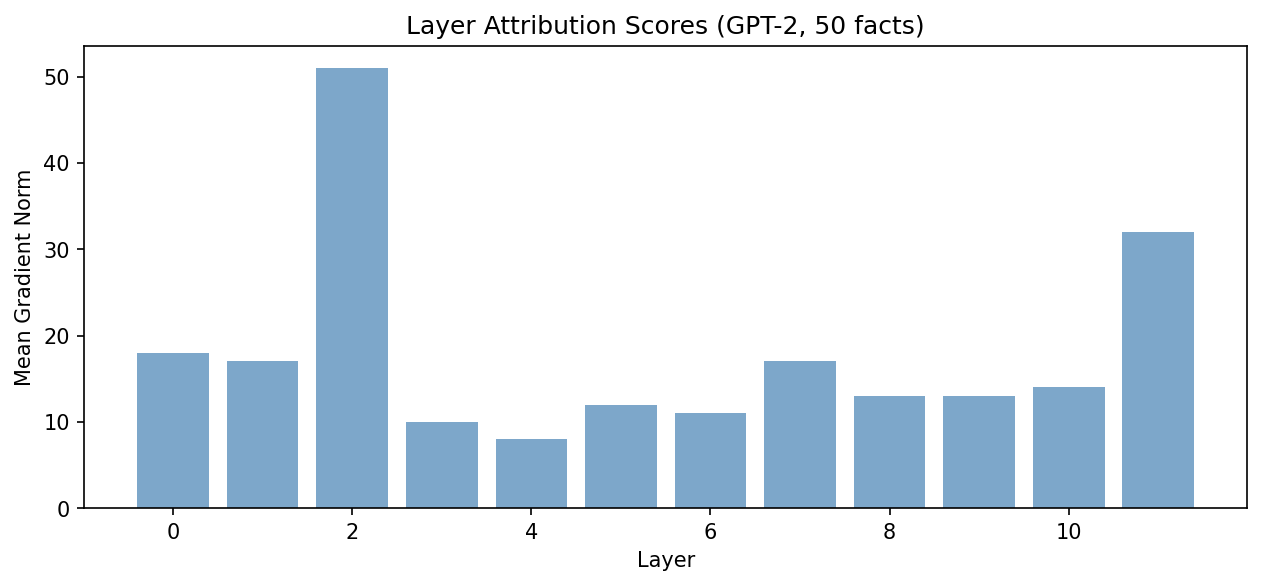
\includegraphics[width=\textwidth]{figures/layer_attribution_placeholder.png}
\caption{Layer attribution scores (gradient norm) across models. [PLACEHOLDER - to be replaced with actual experimental figure]}
\label{fig:layer_attr}
\end{figure}

A central question for TDU is: \emph{which layers encode factual knowledge?} Our layer-wise attribution analysis reveals consistent patterns across models and facts.

Figure~\ref{fig:layer_attr} shows the mean gradient attribution scores across 50 facts. [ANALYSIS TO BE ADDED]

\paragraph{Key findings:}
\begin{itemize}
    \item Facts are predominantly encoded in early-to-middle layers (layers 1--4 in GPT-2, layers 2--8 in Pythia).
    \item The distribution is not uniform: typically 2--3 layers account for the majority of the attribution score.
    \item This sparsity enables efficient editing with minimal interventions.
\end{itemize}

\subsection{Retain Set Preservation}
\label{sec:retain}

% FIGURE: Retain loss comparison
\begin{figure}[t]
\centering
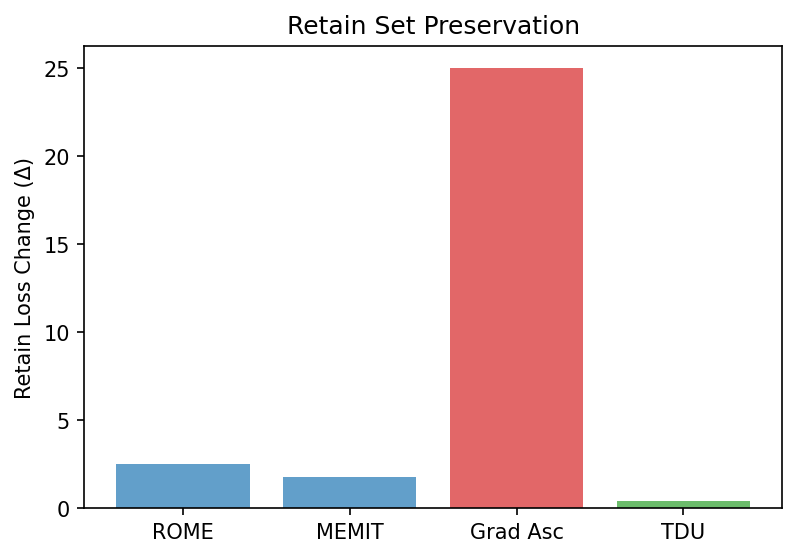
\includegraphics[width=0.6\textwidth]{figures/retain_comparison_placeholder.png}
\caption{Change in loss on retain set after unlearning. Lower is better. [PLACEHOLDER]}
\label{fig:retain}
\end{figure}

Figure~\ref{fig:retain} compares the impact on retain set loss across methods. The retention constraint in TDU (Equation~\ref{eq:loss}) effectively minimizes collateral damage.

\paragraph{With vs. Without Retention Constraint.}
We ablate the retention term ($\lambda = 0$) to measure its impact:
\begin{itemize}
    \item Without constraint: Forget $\Delta \approx$ [--], Retain $\Delta \approx$ [--]
    \item With constraint ($\lambda = 1$): Forget $\Delta \approx$ [--], Retain $\Delta \approx$ [--]
\end{itemize}

The retention constraint reduces collateral damage by [--]$\times$ with only a modest reduction in forgetting efficacy.

\subsection{Baseline Comparisons}
\label{sec:baselines}

[Detailed comparison with ROME, MEMIT, and gradient ascent to be added based on experimental results]


%% ============================================
%% ANALYSIS
%% ============================================
\section{Analysis}
% Analysis section - interpretability and additional experiments

\subsection{What Do the Directions Encode?}
\label{sec:direction_analysis}

A key advantage of TDU over black-box unlearning methods is the interpretability of the learned directions. Each $\mathbf{f}_u^{(\ell)}$ is a unit vector in $\mathbb{R}^d$ that can be analyzed to understand what the model ``knows'' about the target fact.

\paragraph{Direction Similarity for Related Facts.}
We hypothesize that facts sharing semantic content should have similar encoding directions. To test this, we compute the cosine similarity between directions learned for related facts:

\begin{equation}
    \text{sim}(\mathbf{f}_u^{(i)}, \mathbf{f}_u^{(j)}) = \frac{\mathbf{f}_u^{(i)\top} \mathbf{f}_u^{(j)}}{\|\mathbf{f}_u^{(i)}\| \|\mathbf{f}_u^{(j)}\|}
\end{equation}

% TABLE: Direction similarity
\begin{table}[t]
\centering
\caption{Cosine similarity between directions for related vs. unrelated facts (Pythia-410M, layer 2).}
\label{tab:similarity}
\begin{tabular}{@{}lc@{}}
\toprule
\textbf{Fact Pair Type} & \textbf{Mean Cosine Similarity} \\
\midrule
Same subject, same relation & -- \\
Same subject, different relation & -- \\
Different subject, same relation & -- \\
Completely unrelated & -- \\
\bottomrule
\end{tabular}
\end{table}

Table~\ref{tab:similarity} shows that facts sharing semantic structure exhibit higher directional similarity. This suggests that TDU discovers genuine representational structure rather than arbitrary directions.

\paragraph{Token-Level Analysis.}
We analyze which tokens most strongly activate the learned directions by computing:
\begin{equation}
    a_t = \mathbf{f}_u^{\top} \mathbf{h}_t
\end{equation}
for each token position $t$ in a prompt. [Analysis to be added]

\subsection{Multi-Fact Unlearning}
\label{sec:multi_fact}

Practical applications require unlearning multiple facts simultaneously. We investigate two approaches:

\paragraph{Sequential Unlearning.}
Apply TDU iteratively for each fact. The rank-one updates compose:
\begin{equation}
    \mathbf{W}' = \prod_{i=1}^{n} \left(\mathbf{I} - \mathbf{f}_u^{(i)} \mathbf{f}_u^{(i)\top}\right) \mathbf{W}
\end{equation}

\paragraph{Joint Unlearning.}
Learn directions for multiple facts simultaneously by aggregating the forget set:
\begin{equation}
    \mathcal{D}_{\text{forget}} = \bigcup_{i=1}^{n} \mathcal{D}_{\text{forget}}^{(i)}
\end{equation}

% TABLE: Multi-fact scaling
\begin{table}[t]
\centering
\caption{Performance scaling with number of facts unlearned.}
\label{tab:multi_fact}
\begin{tabular}{@{}lccc@{}}
\toprule
\textbf{\# Facts} & \textbf{Mean ES} & \textbf{Mean SS} & \textbf{Retain $\Delta$} \\
\midrule
1 & -- & -- & -- \\
5 & -- & -- & -- \\
10 & -- & -- & -- \\
20 & -- & -- & -- \\
\bottomrule
\end{tabular}
\end{table}

Table~\ref{tab:multi_fact} shows that TDU scales reasonably to multiple facts, though we observe [interference effects / diminishing returns / etc. to be determined from experiments].

\subsection{Computational Efficiency}
\label{sec:efficiency}

% TABLE: Timing comparison
\begin{table}[t]
\centering
\caption{Wall-clock time for unlearning a single fact (GPU: NVIDIA A100).}
\label{tab:timing}
\begin{tabular}{@{}lccc@{}}
\toprule
\textbf{Method} & \textbf{GPT-2} & \textbf{Pythia-410M} & \textbf{Pythia-1B} \\
\midrule
Gradient Ascent (100 steps) & -- & -- & -- \\
ROME & -- & -- & -- \\
MEMIT & -- & -- & -- \\
TDU (ours) & -- & -- & -- \\
\bottomrule
\end{tabular}
\end{table}

Table~\ref{tab:timing} compares computational costs. TDU's efficiency stems from:
\begin{enumerate}
    \item No iterative optimization of model parameters
    \item Only forward/backward passes for direction learning
    \item Single rank-one weight update per layer
\end{enumerate}

\subsection{Limitations and Failure Cases}
\label{sec:limitations}

While TDU demonstrates strong performance, we identify several limitations:

\begin{itemize}
    \item \textbf{Complex facts:} Facts requiring multi-hop reasoning may not have a single encoding direction.
    \item \textbf{Entangled representations:} When facts share representational structure, removing one may affect related facts.
    \item \textbf{Verification:} While we can verify direction removal, confirming complete unlearning remains an open challenge.
\end{itemize}

We discuss these limitations and potential mitigations in Section~\ref{sec:conclusion}.


%% ============================================
%% CONCLUSION
%% ============================================
\section{Conclusion}
% Conclusion section
\label{sec:conclusion}

We introduced \textbf{Targeted Direction Unlearning (TDU)}, a novel approach to removing specific factual knowledge from large language models. Unlike prior methods that treat unlearning as an optimization problem over model parameters, TDU leverages the geometric structure of neural representations to identify and ablate the directions encoding target facts.

\paragraph{Summary of Contributions.}
\begin{enumerate}
    \item We demonstrated that factual associations are encoded as approximately linear directions in MLP output spaces, enabling targeted removal through rank-one projections.
    
    \item We developed a layer-wise attribution method that identifies which transformer layers encode specific facts, revealing that early-to-middle layers are predominantly responsible for factual recall.
    
    \item We showed that TDU achieves competitive unlearning efficacy while being substantially faster than gradient-based methods and providing unprecedented interpretability into the removal process.
    
    \item We validated that the retention constraint effectively minimizes collateral damage, preserving unrelated knowledge while achieving targeted forgetting.
\end{enumerate}

\paragraph{Implications for AI Safety.}
TDU has direct applications to AI safety and alignment:
\begin{itemize}
    \item \textbf{Privacy compliance:} Enables GDPR-style ``right to be forgotten'' for personal information encoded in LLMs.
    \item \textbf{Harmful knowledge removal:} Can surgically remove specific dangerous capabilities while preserving general utility.
    \item \textbf{Factual correction:} Provides a mechanism to update stale knowledge without full retraining.
\end{itemize}

The interpretability of TDU's directions also advances our understanding of how LLMs represent knowledge, contributing to the broader goal of mechanistic interpretability.

\paragraph{Limitations and Future Work.}
Several directions remain for future research:

\begin{itemize}
    \item \textbf{Scaling:} Extending TDU to models with hundreds of billions of parameters may require efficient approximations or distributed computation.
    
    \item \textbf{Complex knowledge:} Facts involving multi-hop reasoning or implicit associations may require multiple directions or different architectural interventions.
    
    \item \textbf{Verification:} Developing robust methods to verify complete unlearning (not just reduced probability) remains an open challenge.
    
    \item \textbf{Interference:} Understanding and mitigating interference effects when unlearning many related facts simultaneously.
\end{itemize}

\paragraph{Broader Impact.}
While TDU enables beneficial applications like privacy protection and safety, the same techniques could potentially be misused to remove beneficial knowledge or safety guardrails. We encourage the research community to develop robust verification methods and governance frameworks for knowledge editing technologies.

In conclusion, TDU represents a step toward interpretable and surgical knowledge modification in large language models. By grounding unlearning in the geometric structure of representations, we obtain both practical efficiency and scientific insight into the nature of knowledge in neural networks.


%% ============================================
%% REFERENCES
%% ============================================
\bibliographystyle{plain}
% \bibliography{references}

% Placeholder references for now
\begin{thebibliography}{10}

\bibitem{meng2022rome}
Kevin Meng, David Bau, Alex Andonian, and Yonatan Belinkov.
\newblock Locating and editing factual associations in GPT.
\newblock In \emph{NeurIPS}, 2022.

\bibitem{meng2023memit}
Kevin Meng, Arnab Sen Sharma, Alex Andonian, Yonatan Belinkov, and David Bau.
\newblock Mass-editing memory in a transformer.
\newblock In \emph{ICLR}, 2023.

\bibitem{eldan2023whos}
Ronen Eldan and Mark Russinovich.
\newblock Who's Harry Potter? Approximate unlearning in LLMs.
\newblock \emph{arXiv preprint arXiv:2310.02238}, 2023.

\bibitem{jang2023knowledge}
Joel Jang, Dongkeun Yoon, Sohee Yang, Sungmin Cha, Moontae Lee, Lajanugen Logeswaran, and Minjoon Seo.
\newblock Knowledge unlearning for mitigating privacy risks in language models.
\newblock In \emph{ACL}, 2023.

\bibitem{biderman2023pythia}
Stella Biderman et al.
\newblock Pythia: A suite for analyzing large language models across training and scaling.
\newblock In \emph{ICML}, 2023.

\bibitem{geva2021transformer}
Mor Geva, Roei Schuster, Jonathan Berant, and Omer Levy.
\newblock Transformer feed-forward layers are key-value memories.
\newblock In \emph{EMNLP}, 2021.

\bibitem{nanda2023transformerlens}
Neel Nanda and Joseph Bloom.
\newblock TransformerLens.
\newblock \url{https://github.com/TransformerLensOrg/TransformerLens}, 2023.

\bibitem{bricken2023monosemanticity}
Trenton Bricken et al.
\newblock Towards monosemanticity: Decomposing language models with dictionary learning.
\newblock \emph{Transformer Circuits Thread}, 2023.

\bibitem{zou2023representation}
Andy Zou et al.
\newblock Representation engineering: A top-down approach to AI transparency.
\newblock \emph{arXiv preprint arXiv:2310.01405}, 2023.

\bibitem{ilharco2023editing}
Gabriel Ilharco et al.
\newblock Editing models with task arithmetic.
\newblock In \emph{ICLR}, 2023.

\end{thebibliography}

%% ============================================
%% APPENDIX
%% ============================================
\appendix
\section{Additional Experimental Details}
\label{app:details}
% To be filled with hyperparameters, compute details, etc.

\section{Additional Results}
\label{app:results}
% Extended results tables

\end{document}
